\clearpage
\section{Deadbeat}

El objetivo del controlador Deadbeat es cancelar la dinámica del sistema para asegurar que este llegue a la referencia en $N$ pasos, siendo $N$ el retardo total del sistema en tiempo discreto. Debido a la naturaleza de este objetivo, el control Deadbeat es inherentemente discreto, por lo que se analizará como tal.

\begin{figure}[H]
  \begin{center}
    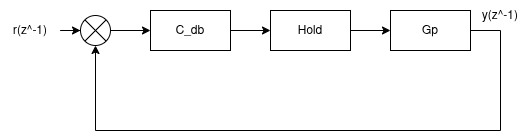
\includegraphics[width=0.8\textwidth]{figures/db.png}
  \end{center}
  \caption{Bloques Deadbeat}\label{bloques-deadbeat}
\end{figure}
Se plantea la planta discretizada, considerando el retardo total del sistema (retenedor de orden cero y tiempo muerto físico):
\[
  G_p(z^{-1}) = \frac{\beta z^{-(N+1)}}{1 - \alpha z^{-1}}
\]

Para garantizar la causalidad, la función de transferencia a lazo cerrado debe contemplar este retardo mínimo exigible:
\[
  H_{LC}(z^{-1}) = z^{-(N+1)}
\]

Partiendo de la ecuación general del controlador:
\[
  C_{dB}(z^{-1}) = \frac{H_{LC}(z^{-1})}{1 - H_{LC}(z^{-1})}\frac{1}{G_p(z^{-1})}
\]

Sustituyendo $H_{LC}(z^{-1})$ y $G_p(z^{-1})$:
\[
  C_{dB}(z^{-1}) = \left( \frac{z^{-(N+1)}}{1 - z^{-(N+1)}} \right) \left( \frac{1 - \alpha z^{-1}}{\beta z^{-(N+1)}} \right)
\]

Los términos $z^{-(N+1)}$ del numerador y denominador se cancelan directamente:
\[
  C_{dB}(z^{-1}) = \frac{1 - \alpha z^{-1}}{\beta(1 - z^{-(N+1)})}
\]

Aplicando la relación $\frac{u(z^{-1})}{e(z^{-1})}$:
\[
  \frac{u(z^{-1})}{e(z^{-1})} = \frac{1 - \alpha z^{-1}}{\beta (1 - z^{-(N+1)})}
\]

Despejando cruzado:
\[
  u(z^{-1}) \cdot \beta (1 - z^{-(N+1)}) = e(z^{-1}) \cdot (1 - \alpha z^{-1})
\]
\[
  \beta u(z^{-1}) - \beta z^{-(N+1)} u(z^{-1}) = e(z^{-1}) - \alpha z^{-1} e(z^{-1})
\]

Aplicando la transformada Z inversa para obtener la ecuación de diferencias:
\[
  \beta u_k - \beta u_{k-(N+1)} = e_k - \alpha e_{k-1}
\]

Finalmente, despejando la acción de control actual $u_k$:
\[
  u_k = u_{k-N-1} + \frac{1}{\beta}e_k - \frac{\alpha}{\beta}e_{k-1}
\]
